\section{Event Reconstruction}
The event reconstruction software has been designed and developed within the CLARA framework.
The reconstruction of events for CLAS12 is separated into micro-services that run data processing algorithms.

The data reader services accesses the decoded data stored in a tablular structure,
called ``bank'', according to
sector, layer, component, ADC/TDC and order (corresponding to left or right PMTs). Each entry for decoded
detector hits is a row in a bank.  Similar bank structures are created at the decoding stage for the
various information needed for event reconstruction, such as hits, clusters, tracks, etc.

The reconstruction micro-services that run event reconstruction algorithms, pertaining to
the subsystems of the CLAS12 detector, fill these banks
that are subsequently appended and written out to a file by a data-persistency micro-service.

The services running the reconstruction algorithms access the various banks (transient data) as input
and produce output banks needed for the subsequent algorithms in the reconstruction chain.
The order of the services depend on the reconstruction sequence.  Some services can run in parallel while others
need the reconstruction output provided by the preceeding ones.
For instance hit-based for the central (CVT service) and for forward (DCHB service) tracking
can run in parallel, while time-based tracking (DCTB) must come after the event builder service
that gathers the output from the various banks run prior to using timing information which requires
the determination of the event start time using the time-of-flight and calorimeters output.
An  overview of the reconstruction application service composition is shown in figures~\ref{fig:clara-overview} and~\ref{fig:services}.


%%%%%%%%%%%%%%%%%%%%%%%%%%%%%%%%%%%%%%%%%%%%%%%%%%%%%%%%%%

\begin{figure*}
\centering
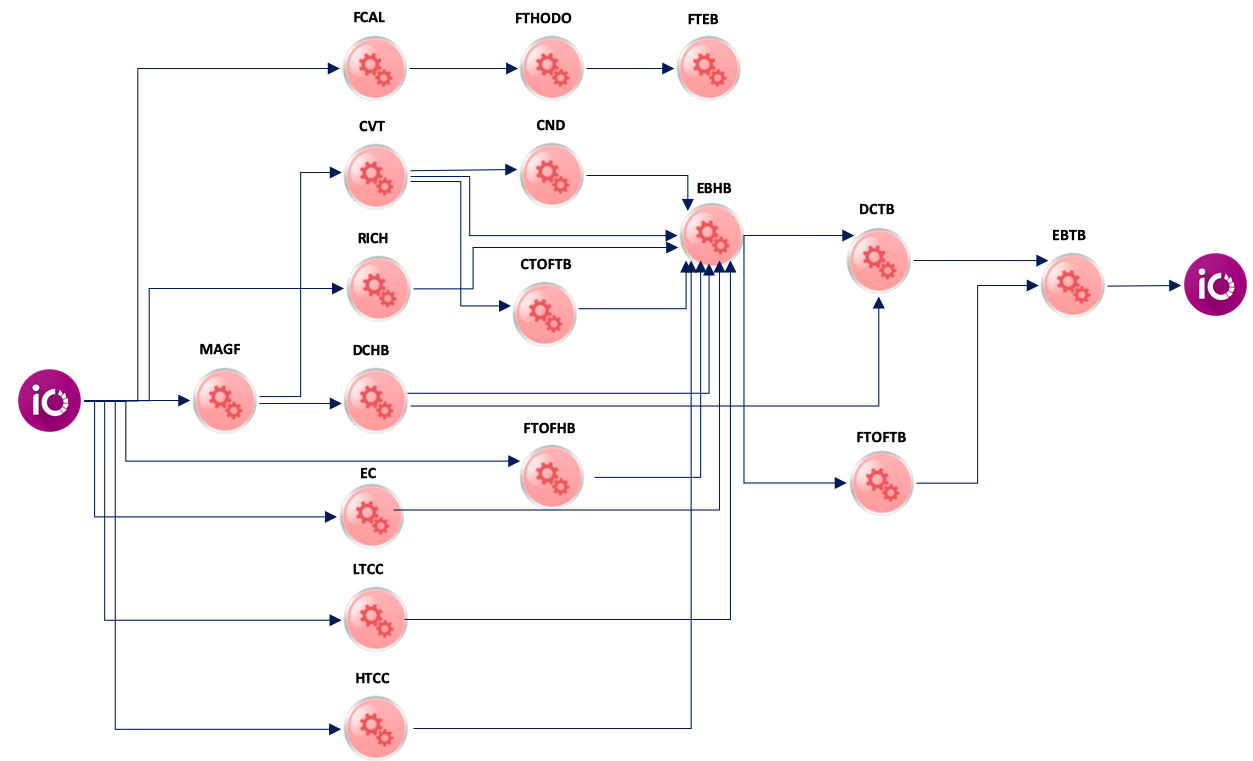
\includegraphics[width=0.6\textwidth]{pics/ServiceComposition.png}
\caption{CLAS12 reconstruction application service composition in case of sub-event level parallelization.
In this case within the event different detector component reconstruction services are processing in parallel.}
\label{fig:services}
\end{figure*}


%%%%%%%%%%%%%%%%%%%%%%%%%%%%%%%%%%%%%%%%%%%%%%%%%%%%%%%%%%%
